\documentclass[12pt,letterpaper,noanswers]{exam}
\usepackage[usenames,dvipsnames,svgnames,table]{xcolor}
\usepackage[margin=0.9in]{geometry}
\renewcommand{\familydefault}{\sfdefault}
\usepackage{multicol}
\pagestyle{head}
\header{AM 111 Class 10}{}{Piecewise interpolation, p.\thepage}
\runningheadrule
\headrule
\usepackage{siunitx}
\usepackage{graphicx} % more modern
\usepackage{amsmath} 
\usepackage{amssymb} 
\usepackage{hyperref}
\usepackage{tcolorbox}
\usepackage{enumitem}
\def\mbf{\mathbf}
\newcommand{\vc}[1]{\boldsymbol{#1}}
\def\dsst{\displaystyle}
\DeclareMathOperator*{\argmin}{arg\,min} % thin space, limits underneath in displays


\begin{document}
 \pdfpageheight 11in 
  \pdfpagewidth 8.5in

\noindent 

\section*{Preliminaries}

\begin{itemize}
\itemsep0pt
\item The problem set is due on Friday at 5pm (submit via Gradescope: include pdfs of all code/output on Gradescope.  Upload any source code to Canvas).
\item The problem set includes some ``time permitting'' problems.  If your total time spent on the course outside of class reaches 10 hours in the week then you are encouraged to skip problems.  If you are not in that situation, you are expected to complete the problems.
\item If you need guidance or help on the problem set, post to Ed.
%\item There will be a skill check in class during the next class.  The problem info is below.
\item Quiz info is on Canvas.
\item There is no problem set the week of the quiz.
\end{itemize}



\noindent\textbf{Big picture}

Today: Algorithms for finding a piecewise polynomial that directly passes through data points.

\vspace{0.2cm}
\hrule
\vspace{0.2cm}

\noindent \textbf{Skill check practice}
\begin{questions}
\item 
% Sauer \S 3.4 Q1
Decide whether the equations form a cubic spline.

\[S(x) = \left\{\begin{array}{l l}
x^3 + x - 1 & \text{on }[0,1] \\
-(x-1)^3 + 3(x-1)^2 + 3(x-1) + 1 & \text{on }[1,2] \\
\end{array}\right.\]

\item The skill from the Class 07 handout (Skill Check C08).
\end{questions}


\vspace{0.2cm}
\hrule
\vspace{0.2cm}

\noindent \textbf{Skill check solution}
\begin{questions}
\item 

$S_1(1) = 1+1-1 = 1$

$S_2(1) = 0 + 0 + 0 + 1 = 1$

So $S(x)$ is continuous.

$S_1'(x) = 3x^2 + 1$ and $S_2'(x) = -3(x-1)^2 + 6(x-1) + 3$.

$S_1'(1) = 3 + 1 = 4$

$S_2'(1) = 0 + 0 + 3$

So $S'(x)$ is not continuous and $S(x)$ is not a cubic spline.

\item See the past handout.
\end{questions}
\vspace{0.2cm}
\hrule
\vspace{0.2cm}

\noindent \textbf{Teams}
\begin{multicols}{3}
1. Eletria, Benjamin, Marissa

2. Cameron, Basil, Emma

3. RH, Eric, Esmé

4. Nini, Ray, Dani

5. Jack, Mina, Ivonne

6. Alex, KevinG, Shang

7. Jessica, Johan, Tom

8. Nina, Robert, Padraig

9. KevinC, Alex, Eli

10.  Aidan, Daniyal, Zachary

11. Ghedion, JuliaK, JuliaM

12. Mack, Brian

13. Caitlin, Sophie

\end{multicols}

\subsection*{Solving a tridiagonal matrix}


\begin{tcolorbox}
A matrix of the form \[\left[\begin{array}{ c c c c c c } 
b_1 & c_1 &  &  & & 0 \\
a_2 & b_2 & c_2 &  &  &  \\
 & a_3 & \ddots & \ddots &  &  \\
 &  &\ddots &  &  & \\
  &  & &  &  & c_{N-1}\\
0 & & & & a_N & b_N
\end{array}\right]\]

is called \textbf{tridiagonal}
\end{tcolorbox}

\begin{enumerate}[resume=classQ]
\item Consider the system \[\left[\begin{array}{c c c c}
1 & 2 & 0 & 0 \\
2 & 3 & 4 & 0 \\
0 & 1 & 7 & 3\\
0 & 0 & 4 & 2
\end{array}\right]\vc{x} = \left[\begin{array}{c} 
1 \\ 6 \\ 7 \\ 2
\end{array}\right]\]

\begin{parts}
\item Eliminate the $a_i$ elements.  Divide the first row by $b_1$, multiply by $a_2$, and subtract if from the second row.  Continue with this procedure to create an upper triangular matrix.
\vfill

\item How many addition, subtraction, multiplication, division operations did this require?  These are basic floating point operations, FLOPs.
\vspace{1cm}

\item Use back substitution to solve your resulting matrix.
\vfill

\item Again count the FLOPs.

\end{parts}

This algorithm for solving a tridiagonal system is $\mathcal{O}(N)$.
\end{enumerate}


\href{https://edsonmarine.com/set-of-six-bronze-spline-weights/}{Splines for sale}

\subsection*{B-splines}

(Heath \S 7.4.3)

\begin{tcolorbox}
Can a cubic spline be represented as a linear combination of basis functions?

This \textbf{B-splines} form a basis for the splines of a given degree.
\end{tcolorbox}

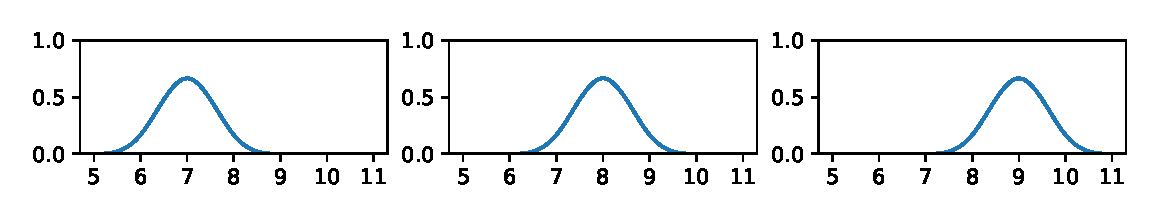
\includegraphics[width=\textwidth]{img/C10bsplinecubes.eps}

\begin{enumerate}[resume=classQ]
\item Three B-splines of degree $3$ are shown above.  

The knots were set to $1,2,3,...,40$.  $B_5^3(x)$, $B_6^3(x)$, $B_7^3(x)$ are the B-splines shown (from left to right).
\begin{parts}
\item Based on these graphs, identify the range of $x$ for which $B_i^3(x)$ is nonzero.
\vspace{1cm}

\item Based on your guess in (a), at $x = 8$ which B-splines will be non-zero?
\vspace{1cm}

\end{parts}
\item Let $x_1, ... x_N$ form the knots for a cubic spline interpolant.

At $x_1$, which B-splines will be nonzero?  What additional knots are needed so that these B-splines can be defined?
\vspace{1in}

\end{enumerate}
\begin{tcolorbox}
Let $x_1, ... x_N$ form the knots for a cubic spline interpolant.
\begin{itemize}
\itemsep0pt
    \item For convenience, assume the set of knots is infinite, $\hdots < x_{-2} < x_{-1}< x_0 < x_1 < \hdots$
    \item The additional knots can be arbitrarily defined outside of the inverval $[x_1, x_N]$.
\end{itemize}
\end{tcolorbox}
\begin{tcolorbox}
The B-splines of degree $3$ have the following properties:
\begin{itemize}
    \item $B_i^3(x)$ has \textbf{local support}: $ \begin{array}{l l}
    B_i^3(x) = 0 & x<x_i \text{ or }x>x_{i+4} \\
    B_i^3(x) >0 & x_i < x < x_{i+4}
    \end{array}$
        \item For all $x$, $\displaystyle\sum\limits_{i=-\infty}^\infty B_i^3(x) = 1$
    \end{itemize}
\end{tcolorbox}
\begin{tcolorbox}
\begin{itemize}

    \item The set of functions $\left\{B_{-2}^3,...,B_{N-1}^3\right\}$ is linearly independent on the interval $[x_1,x_N]$
    \item The set of functions $\left\{B_{-2}^3,...,B_{N-1}^3\right\}$ spans the set of all splines of degree $3$ having knots $x_1,...,x_N$
\end{itemize}
\end{tcolorbox}
\begin{enumerate}[resume=classQ]
\item You have data $\left\{(x_i,y_i)_{i = 1}^{20} \right\}$ with a cubic spline interpolant $P(x)$.

Assume that you have found the coefficients $c_{-2}, c_{-1}, ..., c_{N-1}$ to be able to write $P(x) = c_{-2}B_{-2}^3(x) + c_{-1}B_{-1}^3(x) + \hdots + c_{N-1}B_{N-1}^3(x)$.  

You remeasure the data for $x_8$ and find a new value for $y_8$.  Which $c_i$ need to change to create $Q(x)$, a cubic spline interpolant for your new data?
\vspace{1in}

\end{enumerate}



\begin{tcolorbox}
B-splines are defined via recursion.

\[B_i^0(x) = \left\{\begin{array}{l l}
1 & \text{if }x_i\leq x < x_{i+1} \\
0 & \text{otherwise}
\end{array}\right.\]

and

\[B_i^k(x) = v_i^k(x)B_i^{k-1}(x) +\left(1-v_{i+1}^k(x)\right)B_{i+1}^{k-1}(x), \text{ where } v_i^k(x) = \dfrac{x-x_i}{x_{i+k}-x_i}\] 



Plugging in $k=3$, we have
$\displaystyle B_i^3(x) = \dfrac{x - x_i}{x_{i+3}-x_i} B_i^2(x) + \dfrac{x_{i+4}-x}{x_{i+4}-x_{i+1}}B_{i+1}^2(x)$

\end{tcolorbox}
\begin{enumerate}[resume=classQ]
\item Let the knots $x_i$ be set by $x_i = i$.  Sketch $B_3^0(x)$.  Let your $x$-axis be $1\leq x \leq 6$.
\vspace{1.5in}

\item Use the definition of $B_i^k(x)$ to find $B_3^1(x)$.

Add a sketch of $B_3^1(x)$ to your plot above.

\end{enumerate}

\texttt{scipy.interpolate.splrep} finds a B-spline representation.

\texttt{scipy.interpolate.splev} evaluates a spline interpolation represented via B-splines.
\end{document}